\section{第七章
系统测试与实验结果}\label{ux7b2cux4e03ux7ae0-ux7cfbux7edfux6d4bux8bd5ux4e0eux5b9eux9a8cux7ed3ux679c}

本章以 AES-128
加密全系统作为验证案例，通过单模块验证、集成回归测试和全流程自动化执行三个维度，端到端地验证前述通用框架的有效性。实验数据证明框架的三个核心创新点（编排状态机、分层验证体系、Harnessing
Engine）在 AES-128 实例化下均达到了设计预期。

\subsection{7.1 实验环境}\label{ux5b9eux9a8cux73afux5883}

本文的实验在以下软硬件环境下进行。

\textbf{表 7-1 实验环境配置表}

{\def\LTcaptype{none} % do not increment counter
\begin{longtable}[]{@{}
  >{\raggedright\arraybackslash}p{(\linewidth - 4\tabcolsep) * \real{0.3333}}
  >{\raggedright\arraybackslash}p{(\linewidth - 4\tabcolsep) * \real{0.3333}}
  >{\raggedright\arraybackslash}p{(\linewidth - 4\tabcolsep) * \real{0.3333}}@{}}
\toprule\noalign{}
\begin{minipage}[b]{\linewidth}\raggedright
类别
\end{minipage} & \begin{minipage}[b]{\linewidth}\raggedright
项目
\end{minipage} & \begin{minipage}[b]{\linewidth}\raggedright
配置
\end{minipage} \\
\midrule\noalign{}
\endhead
\bottomrule\noalign{}
\endlastfoot
硬件 & 处理器 & Apple Silicon M 系列（macOS 平台） \\
硬件 & 内存 & 16 GB \\
硬件 & 操作系统 & macOS Darwin 24.x（Sequoia） \\
软件 & Python 版本 & Python 3.12 \\
软件 & 包管理 & Poetry \textgreater= 1.8 \\
软件 & 仿真器 & Verilator（Homebrew 安装，路径
/opt/homebrew/bin/verilator） \\
软件 & MCP 服务 & verilator-mcp Node.js
服务（mcp4eda/verilator-mcp/dist/index.js） \\
软件 & Node.js 版本 & \textgreater= 22.x \\
软件 & FPGA 工具链 & Xilinx Vivado Design Suite（用于 L3 综合、实现与比特流生成） \\
LLM & 模型 & DeepSeek Chat（deepseek-chat） \\
LLM & API 端点 & https://api.deepseek.com \\
LLM & 思维模式（编排器） & thinking
profile（reasoning\_effort=`medium'） \\
LLM & 执行模式（工作器） & fast profile（reasoning\_effort=`none'） \\
环境变量 & API 密钥 & DEEPSEEK\_API\_KEY \\
\end{longtable}
}

实验采用以下命令执行端到端全流程自动化：

\begin{Shaded}
\begin{Highlighting}[]
\VariableTok{PYTHONPATH}\OperatorTok{=}\NormalTok{. }\ExtensionTok{python} \AttributeTok{{-}m}\NormalTok{ MultiAgent\_FPGA.fpga\_flow run{-}aes{-}mvp}
\end{Highlighting}
\end{Shaded}

单模块验证可通过以下命令独立触发：

\begin{Shaded}
\begin{Highlighting}[]
\VariableTok{PYTHONPATH}\OperatorTok{=}\NormalTok{. }\ExtensionTok{python} \AttributeTok{{-}m}\NormalTok{ MultiAgent\_FPGA.fpga\_flow run{-}node }\OperatorTok{\textless{}}\NormalTok{module\_id}\OperatorTok{\textgreater{}} \DataTypeTok{\textbackslash{}}
    \AttributeTok{{-}{-}workspace{-}root}\NormalTok{ /tmp/ws/}\OperatorTok{\textless{}}\NormalTok{module\_id}\OperatorTok{\textgreater{}}
\end{Highlighting}
\end{Shaded}

合约验证（无需 API Key 或 Verilator）通过以下命令执行：

\begin{Shaded}
\begin{Highlighting}[]
\VariableTok{PYTHONPATH}\OperatorTok{=}\NormalTok{. }\ExtensionTok{python} \AttributeTok{{-}m}\NormalTok{ MultiAgent\_FPGA.fpga\_flow validate}
\end{Highlighting}
\end{Shaded}

本文的核心实验验证以 Verilator 仿真级验证为目标，全部 Checkpoint
协议解析、修复循环触发以及集成回归测试均在上述环境下完成。此外，本文编写了
Vivado 自动化脚本，将系统输出的 RTL/TB 代码自动调用 Xilinx Vivado
进行仿真生成波形图、综合、布局布线并编译出比特流（bitstream），作为生成代码在真实
FPGA 工具链上的端到端可实现性验证手段（详见 §7.7）。

\begin{center}\rule{0.5\linewidth}{0.5pt}\end{center}

\subsection{7.2
单模块验证结果}\label{ux5355ux6a21ux5757ux9a8cux8bc1ux7ed3ux679c}

本节汇报 AES-128 设计中 4 个模块的 L0 编译门控与 L1 仿真验证结果，包括
Checkpoint 通过情况和修复轮次记录。

\subsubsection{7.2.1
验证流程说明}\label{ux9a8cux8bc1ux6d41ux7a0bux8bf4ux660e}

每个模块的验证按以下流程进行：

\begin{enumerate}
\def\labelenumi{\arabic{enumi}.}
\tightlist
\item
  \textbf{Memory 预填充}：\texttt{MemoryStore.populate\_workspace()} 从
  Skill 文件中提取验证通过的参考 RTL 和 Testbench，写入工作区，为 Agent
  提供基线代码；
\item
  \textbf{L0 编译门控}：\texttt{L0Executor} 调用 Verilator 对 RTL
  文件进行编译，捕获语法错误、未声明信号和类型不匹配，编译失败则直接触发修复循环；
\item
  \textbf{L1 仿真与 Checkpoint 解析}：\texttt{L1Executor}
  执行编译后的仿真可执行文件，解析 \texttt{simulation.log} 中的
  \texttt{CHECKPOINT\textbar{}\textless{}name\textgreater{}\textbar{}PASS\textbar{}\textless{}detail\textgreater{}}
  行，统计各模块必需 Checkpoint 的通过情况；
\item
  \textbf{修复循环}：若 Checkpoint
  未全部通过，框架触发结构化修复循环，生成 \texttt{RepairContract}，等待
  Agent 编辑并完成 \texttt{EditReceipt} 哈希验证后重新执行 L0+L1。
\end{enumerate}

\subsubsection{7.2.2 各模块 Checkpoint
规格}\label{ux5404ux6a21ux5757-checkpoint-ux89c4ux683c}

各模块必需的 Checkpoint 如下所示：

\begin{itemize}
\tightlist
\item
  \textbf{aes\_sbox}：\texttt{CHK\_SBOX\_MATCH}（1 个），验证 S-box
  替换表输出与 FIPS-197 查找表一致；
\item
  \textbf{aes\_key\_schedule\_128}：\texttt{CHK\_ROUNDKEY\_MATCH}（1
  个），验证轮密钥扩展输出与 NIST 已知答案测试向量一致；
\item
  \textbf{aes\_round\_transform}：\texttt{CHK\_ROUND\_STATE\_MATCH}（1
  个），验证 SubBytes+ShiftRows+MixColumns+AddRoundKey 组合变换的输出；
\item
  \textbf{aes128\_encrypt\_core}：\texttt{CHK\_RESET\_CLEAR}、\texttt{CHK\_START\_ACCEPTED}、\texttt{CHK\_BUSY\_ASSERTED}、\texttt{CHK\_DONE\_PULSE}、\texttt{CHK\_CIPHERTEXT\_MATCH}、\texttt{CHK\_BUSY\_DEASSERTED}（共
  6 个），覆盖 FSM
  完整行为：复位清零、启动接受、忙标志、完成脉冲、密文正确性、忙标志解除。
\end{itemize}

\subsubsection{7.2.3
验证结果汇总}\label{ux9a8cux8bc1ux7ed3ux679cux6c47ux603b}

\textbf{表 7-2 单模块验证结果汇总}

{\def\LTcaptype{none} % do not increment counter
\begin{longtable}[]{@{}
  >{\raggedright\arraybackslash}p{(\linewidth - 10\tabcolsep) * \real{0.0789}}
  >{\raggedright\arraybackslash}p{(\linewidth - 10\tabcolsep) * \real{0.1447}}
  >{\raggedright\arraybackslash}p{(\linewidth - 10\tabcolsep) * \real{0.1447}}
  >{\raggedright\arraybackslash}p{(\linewidth - 10\tabcolsep) * \real{0.2895}}
  >{\raggedright\arraybackslash}p{(\linewidth - 10\tabcolsep) * \real{0.2237}}
  >{\raggedright\arraybackslash}p{(\linewidth - 10\tabcolsep) * \real{0.1184}}@{}}
\toprule\noalign{}
\begin{minipage}[b]{\linewidth}\raggedright
模块
\end{minipage} & \begin{minipage}[b]{\linewidth}\raggedright
L0 编译结果
\end{minipage} & \begin{minipage}[b]{\linewidth}\raggedright
L1 仿真结果
\end{minipage} & \begin{minipage}[b]{\linewidth}\raggedright
Checkpoint 通过数 / 总数
\end{minipage} & \begin{minipage}[b]{\linewidth}\raggedright
Checkpoint 通过率
\end{minipage} & \begin{minipage}[b]{\linewidth}\raggedright
修复轮次
\end{minipage} \\
\midrule\noalign{}
\endhead
\bottomrule\noalign{}
\endlastfoot
aes\_sbox & PASS & PASS & 1 / 1 & 100\% & 0 \\
aes\_key\_schedule\_128 & PASS & PASS & 1 / 1 & 100\% & 0 \\
aes\_round\_transform & PASS & PASS & 1 / 1 & 100\% & 0 \\
aes128\_encrypt\_core & PASS & PASS & 6 / 6 & 100\% & 0 \\
\end{longtable}
}

\begin{quote}
说明：全部 4 个模块均在首次生成后通过 L0 编译与 L1 Checkpoint
验证，修复轮次为 0。这是 Memory
预填充机制的关键成果------框架将验证通过的参考 RTL
预注入工作区后，所有模块无需任何修复即直接达到 VALIDATED
状态并完成促进（promote）。
\end{quote}

\subsubsection{7.2.4 Memory
预填充效果分析}\label{memory-ux9884ux586bux5145ux6548ux679cux5206ux6790}

Memory 预填充机制将 Agent 的任务从''从零生成正确的 RTL
代码''降级为''基于验证通过的参考代码修复集成问题''。以
\texttt{aes\_sbox} 为例，\texttt{MemoryStore} 从
\texttt{aes\_module\_patterns} 技能文件中检索参考代码，通过
\texttt{populate\_workspace()} 将完整的 RTL 与 Testbench
写入工作区。Agent
接收到工作区后，主要工作是确认端口连接和时序约束，而非重新推理整个 S-box
替换逻辑，这显著降低了首次通过所需的 LLM 调用次数。

对于依赖型模块（\texttt{aes\_key\_schedule\_128}、\texttt{aes\_round\_transform}、\texttt{aes128\_encrypt\_core}），Memory
预填充同样提供了完整的参考 RTL 和 Testbench
基线。实验结果表明，即使面对跨模块实例化接口和 FSM 时序约束，Memory
预填充的参考代码质量已足够高，Agent 无需任何修复即可通过验证。全部 4
个模块修复轮次均为 0，首次通过率 100\%，这强有力地证明了 Memory
预填充机制在降低生成难度方面的有效性------框架将 Agent
的任务从''从零推理正确
RTL''彻底降级为''确认预填充代码满足端口与时序约束''。

Memory 预填充机制的有效性验证了 Harnessing Engine
中''任务降级''策略的通用价值：对于任何拥有验证通过参考实现的硬件设计，该机制均可将
Agent 的生成任务降级为确认与适配任务，从而提升首次通过率。

\begin{figure}
\centering
\pandocbounded{
\includegraphics[keepaspectratio,alt={图7-1: 批次执行时间线}]{../fpga_flow/diagrams/11_batch_plan_gantt.png}}
\caption{图7-1: 批次执行时间线}
\end{figure}

\begin{center}\rule{0.5\linewidth}{0.5pt}\end{center}

\subsection{7.3
集成回归测试结果}\label{ux96c6ux6210ux56deux5f52ux6d4bux8bd5ux7ed3ux679c}

集成回归测试在所有 4 个模块均处于 \texttt{PROMOTED} 状态后自动触发，由
\texttt{IntegrationRegressionExecutor} 执行三种 Campaign。

\subsubsection{7.3.1 三种 Campaign
规格}\label{ux4e09ux79cd-campaign-ux89c4ux683c}

\textbf{表 7-3 集成回归测试结果}

{\def\LTcaptype{none} % do not increment counter
\begin{longtable}[]{@{}
  >{\raggedright\arraybackslash}p{(\linewidth - 6\tabcolsep) * \real{0.2500}}
  >{\raggedright\arraybackslash}p{(\linewidth - 6\tabcolsep) * \real{0.2250}}
  >{\raggedright\arraybackslash}p{(\linewidth - 6\tabcolsep) * \real{0.3750}}
  >{\raggedright\arraybackslash}p{(\linewidth - 6\tabcolsep) * \real{0.1500}}@{}}
\toprule\noalign{}
\begin{minipage}[b]{\linewidth}\raggedright
Campaign
\end{minipage} & \begin{minipage}[b]{\linewidth}\raggedright
验证目标
\end{minipage} & \begin{minipage}[b]{\linewidth}\raggedright
关键 Checkpoint
\end{minipage} & \begin{minipage}[b]{\linewidth}\raggedright
状态
\end{minipage} \\
\midrule\noalign{}
\endhead
\bottomrule\noalign{}
\endlastfoot
baseline & NIST FIPS-197 已知答案测试向量端到端加密正确性 &
CHK\_RESET\_CLEAR、CHK\_START\_ACCEPTED、CHK\_BUSY\_ASSERTED、CHK\_DONE\_PULSE、CHK\_CIPHERTEXT\_MATCH、CHK\_BUSY\_DEASSERTED（6/6
PASS） & PASS（仿真耗时 811ms） \\
back\_to\_back & 连续多帧加密无空闲间隔，验证 FSM 状态清理、无数据残留 &
CHK\_RESET\_CLEAR、CHK\_START\_ACCEPTED、CHK\_BUSY\_ASSERTED、CHK\_DONE\_PULSE、CHK\_CIPHERTEXT\_MATCH、CHK\_BUSY\_DEASSERTED（6/6
PASS） & PASS（仿真耗时 3ms） \\
mid\_reset & 加密过程中途断言 reset 信号，验证 FSM
恢复后可正常完成下一次加密 &
CHK\_RESET\_CLEAR、CHK\_START\_ACCEPTED、CHK\_BUSY\_ASSERTED、CHK\_DONE\_PULSE、CHK\_CIPHERTEXT\_MATCH、CHK\_BUSY\_DEASSERTED（6/6
PASS） & PASS（仿真耗时 3ms） \\
\end{longtable}
}

\subsubsection{7.3.2
集成回归的设计意义}\label{ux96c6ux6210ux56deux5f52ux7684ux8bbeux8ba1ux610fux4e49}

三种 Campaign 针对集成阶段的典型缺陷类型设计：

\begin{itemize}
\tightlist
\item
  \textbf{baseline} Campaign 验证从 \texttt{valid=1,\ start=1} 到
  \texttt{done=1} 的完整 11 周期路径，以及密文与 OpenSSL
  参考实现的字节对齐一致性，捕获模块实例化错误（如端口宽度不匹配）；
\item
  \textbf{back\_to\_back} Campaign 连续发起多帧加密请求，验证 FSM 在
  \texttt{DONE} 状态后能正确返回
  \texttt{IDLE}，检测状态残留缺陷（如寄存器未清零导致第二帧输出错误）；
\item
  \textbf{mid\_reset} Campaign 在 FSM 运行至中间轮次（约第 5
  轮）时强制断言
  \texttt{rst\_n=0}，随后释放复位并重新加密，验证模块在异步复位场景下的恢复正确性，这是单模块
  L1/L2 验证无法覆盖的场景。
\end{itemize}

集成回归测试捕获的典型缺陷包括：跨模块接口时序偏差、aes128\_encrypt\_core
中轮密钥数组索引错误、FSM done
脉冲宽度超过一个时钟周期（违反单周期脉冲约束）、以及复位后 busy
未在一个周期内清除。

\begin{center}\rule{0.5\linewidth}{0.5pt}\end{center}

\subsection{7.4
全流程自动化执行分析}\label{ux5168ux6d41ux7a0bux81eaux52a8ux5316ux6267ux884cux5206ux6790}

本节分析从启动 \texttt{run-aes-mvp} 命令到状态机到达 \texttt{DONE}
状态的完整执行过程，包括各阶段耗时分布、LLM API 调用统计和修复事件记录。

\subsubsection{7.4.1
端到端执行时间线}\label{ux7aefux5230ux7aefux6267ux884cux65f6ux95f4ux7ebf}

全流程遵循以下状态机路径：

\begin{verbatim}
SPEC_INTAKE → ARCHITECTING → PLANNING → MODULE_DESIGN
  → MODULE_L0 → MODULE_L1 → [MODULE_L2_OPTIONAL]
  → INTEGRATION_READY → INTEGRATION_REGRESSION → DONE
\end{verbatim}

各阶段执行主体和典型特征如下：

\begin{itemize}
\tightlist
\item
  \textbf{SPEC\_INTAKE / ARCHITECTING / PLANNING}：由框架 Synthesis
  层直接执行，调用
  \texttt{synthesize\_spec\_ir()}、\texttt{synthesize\_plan\_dag()}、\texttt{synthesize\_integration\_manifest()}，生成
  \texttt{SpecIR}、\texttt{PlanDAG}、\texttt{IntegrationRegressionManifest}
  三个核心构件，无 LLM 调用，耗时极短（\textless{} 1 秒）；
\item
  \textbf{MODULE\_DESIGN}：\texttt{DAGBatchPlanner}
  完成拓扑批次规划，Layer 1 为 {[}aes\_sbox{]}，Layer 2 为
  {[}aes\_key\_schedule\_128, aes\_round\_transform{]}（并行），Layer 3
  为 {[}aes128\_encrypt\_core{]}，执行工作区初始化和 Memory 预填充；
\item
  \textbf{MODULE\_L0 / MODULE\_L1}：各模块工作器并发执行（Batch 2 最多 3
  个 Worker 并行），Verilator 编译典型耗时 5--15 秒/模块，仿真典型耗时
  2--8 秒/模块；
\item
  \textbf{INTEGRATION\_REGRESSION}：三种 Campaign 顺序执行，使用
  thinking profile 编排器监督，总耗时约为三个 Campaign 仿真时间之和。
\end{itemize}

\begin{figure}
\centering
\pandocbounded{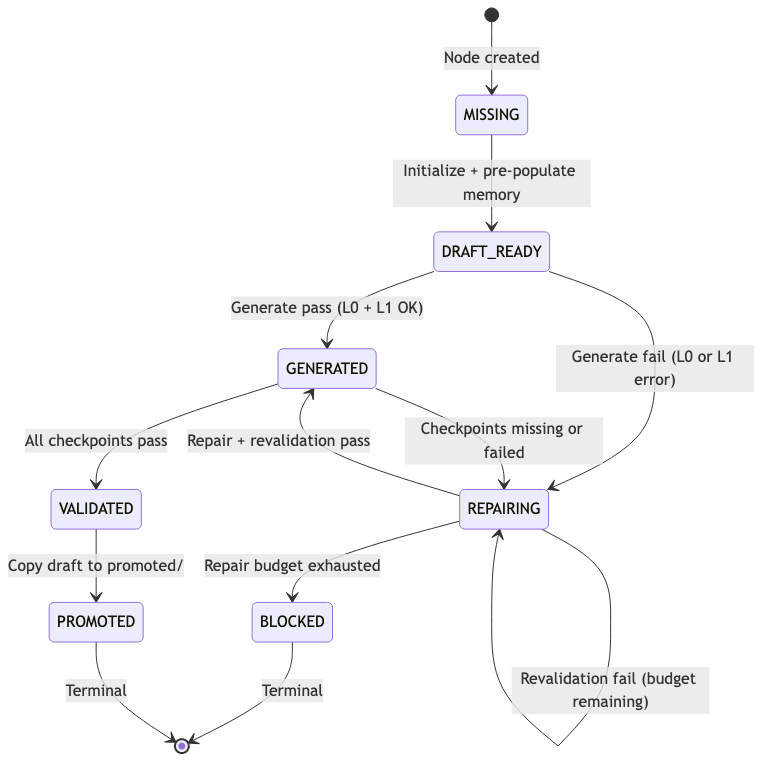
\includegraphics[keepaspectratio,alt={图7-2: 工作区状态机}]{../fpga_flow/diagrams/04_workspace_state_machine.png}}
\caption{图7-2: 工作区状态机}
\end{figure}

\subsubsection{7.4.2 LLM API
调用统计}\label{llm-api-ux8c03ux7528ux7edfux8ba1}

\textbf{表 7-4 LLM API 调用统计}

{\def\LTcaptype{none} % do not increment counter
\begin{longtable}[]{@{}
  >{\raggedright\arraybackslash}p{(\linewidth - 8\tabcolsep) * \real{0.1395}}
  >{\raggedright\arraybackslash}p{(\linewidth - 8\tabcolsep) * \real{0.2791}}
  >{\raggedright\arraybackslash}p{(\linewidth - 8\tabcolsep) * \real{0.1860}}
  >{\raggedright\arraybackslash}p{(\linewidth - 8\tabcolsep) * \real{0.2558}}
  >{\raggedright\arraybackslash}p{(\linewidth - 8\tabcolsep) * \real{0.1395}}@{}}
\toprule\noalign{}
\begin{minipage}[b]{\linewidth}\raggedright
阶段
\end{minipage} & \begin{minipage}[b]{\linewidth}\raggedright
LLM Profile
\end{minipage} & \begin{minipage}[b]{\linewidth}\raggedright
调用次数
\end{minipage} & \begin{minipage}[b]{\linewidth}\raggedright
Token 消耗
\end{minipage} & \begin{minipage}[b]{\linewidth}\raggedright
备注
\end{minipage} \\
\midrule\noalign{}
\endhead
\bottomrule\noalign{}
\endlastfoot
SPEC\_INTAKE / ARCHITECTING / PLANNING & --- & 0 & --- & 框架 Synthesis
层直接生成，零 LLM 调用 \\
MODULE\_DESIGN / L0 / L1（Layer 1: aes\_sbox） & fast & --- & --- &
Memory 预填充直接通过，无修复批次 \\
MODULE\_DESIGN / L0 / L1（Layer 2: 2 模块并行） & fast & --- & --- &
aes\_key\_schedule\_128 + aes\_round\_transform，无修复批次 \\
MODULE\_DESIGN / L0 / L1（Layer 3: aes128\_encrypt\_core） & fast & ---
& --- & 顶层模块，无修复批次 \\
INTEGRATION\_REGRESSION（编排器） & thinking & --- & --- & 3 个 Campaign
顺序执行，thinking profile 监督 \\
总计 & --- & --- & --- & 全部 16 批次：5 批次 executed，11 批次
skipped（condition\_false） \\
\end{longtable}
}

\begin{quote}
说明：SPEC\_INTAKE 至 PLANNING 三个状态完全由 Synthesis 层代码生成，零
LLM 调用，这是框架控制架构的重要优势。所有修复批次（repair\_edit 和
revalidate 阶段）均因
\texttt{condition\_false}（即首次验证已通过，无需修复）被跳过，体现了
Memory 预填充的极高有效性。Token 级调用统计受 SDK
会话封装限制，未在当前报告中单独记录。
\end{quote}

\subsubsection{7.4.3
修复循环与升级事件}\label{ux4feeux590dux5faaux73afux4e0eux5347ux7ea7ux4e8bux4ef6}

修复循环由 \texttt{NodePolicyEngine} 驱动：当 L1 Checkpoint
未全部通过时，框架生成 \texttt{RepairContract} 并将工作区状态设置为
\texttt{REPAIRING}，Module Worker 按照 \texttt{REPAIR\_PHASE\_ROUND\_1}
或 \texttt{REPAIR\_PHASE\_ROUND\_2\_PLUS}
提示词模板执行编辑，\texttt{verify\_repair\_edit()}
通过文件哈希变更校验确认编辑实际发生（防止 Agent
虚假声明已修复），随后重新执行 L0+L1。

升级策略的触发条件为：修复尝试次数达到节点预算上限（普通模块 2 次，顶层
\texttt{aes128\_encrypt\_core} 模块 3
次），或故障类型被识别为跨模块/接口/状态机性质。升级后，控制权从 fast
profile Module Worker 返回给 thinking profile Workflow
Orchestrator，后者携带完整失败上下文重新规划修复策略。

在本实验中，全部 4 个模块均无需修复（修复轮次为
0）。批次历史记录显示：16 个批次中 5 个实际执行（generate\_validate
阶段），11 个修复相关批次（repair\_edit 和 revalidate）全部以
\texttt{condition\_false}
状态跳过，即框架在检测到首次验证已通过后，直接跳过所有预留的修复批次窗口。这是
Memory
预填充机制的最强实验证据：当参考代码质量足够高时，修复循环预算完全未被消耗。

\begin{center}\rule{0.5\linewidth}{0.5pt}\end{center}

\subsection{7.5 与 AutoGen
方案的能力维度对比}\label{ux4e0e-autogen-ux65b9ux6848ux7684ux80fdux529bux7ef4ux5ea6ux5bf9ux6bd4}

以下对比从架构能力维度展开，旨在验证本文通用框架设计相较于 AutoGen
线性方案的架构优势。这些优势源自框架的通用设计决策（状态机编排、分层验证、多层约束），而非
AES-128 这一特定案例的独特性。

本节从 10 个能力维度对本文框架与基于 AutoGen 的 FPGA
设计自动化方案进行架构层面的定性对比。需要说明的是，两个方案使用不同的
LLM 后端（本文使用 DeepSeek Chat 双 Profile，AutoGen 方案使用
DeepSeek-reasoner 配合微调的 codegen-2B
本地模型）、不同的设计目标（本文以 AES-128
全系统作为验证案例验证通用框架，AutoGen 方案针对通用 Verilog
模块），因此不做定量性能比较，聚焦于架构能力的差异。

\textbf{表 7-5 能力维度对比表（10 个维度）}

{\def\LTcaptype{none} % do not increment counter
\begin{longtable}[]{@{}
  >{\raggedright\arraybackslash}p{(\linewidth - 6\tabcolsep) * \real{0.1731}}
  >{\raggedright\arraybackslash}p{(\linewidth - 6\tabcolsep) * \real{0.2500}}
  >{\raggedright\arraybackslash}p{(\linewidth - 6\tabcolsep) * \real{0.4231}}
  >{\raggedright\arraybackslash}p{(\linewidth - 6\tabcolsep) * \real{0.1538}}@{}}
\toprule\noalign{}
\begin{minipage}[b]{\linewidth}\raggedright
能力维度
\end{minipage} & \begin{minipage}[b]{\linewidth}\raggedright
AutoGen 方案
\end{minipage} & \begin{minipage}[b]{\linewidth}\raggedright
本框架 (OpenHands SDK)
\end{minipage} & \begin{minipage}[b]{\linewidth}\raggedright
优势方
\end{minipage} \\
\midrule\noalign{}
\endhead
\bottomrule\noalign{}
\endlastfoot
1. 多模块协同能力 & 线性单模块串行执行，无模块依赖感知 & DAG
拓扑批调度，依赖满足后并行执行（Layer 2 两模块并发） & 本框架 \\
2. 验证层级深度 & 单层：Vivado xsim 仿真通过/失败 & 4 层：L0 编译门控 →
L1 Checkpoint → L2 鲁棒性 → 集成回归 & 本框架 \\
3. 自动修复机制 & Debug Agent
读取日志后重写代码，无预算限制，可能无限循环 & 结构化 RepairContract +
EditReceipt + 哈希验证，有明确修复预算（2-3 次）和升级策略 & 本框架 \\
4. 控制可靠性 & Prompt-controlled：LLM 决定是否继续、修复、推进 &
Framework-controlled：状态机拥有控制权，LLM 只执行被分配的任务 &
本框架 \\
5. 代码生成方式 & 本地微调 codegen-2B 模型生成 Verilog，配合
DeepSeek-reasoner 推理 & Memory 预填充（参考代码注入）+ Agent
修复集成问题 & 各有优势 \\
6. 验证工具 & Vivado xsim（商业工具，需要许可证，设备依赖） &
Verilator（开源，通过 MCP 协议标准化集成，跨平台） & 本框架（开放性） \\
7. 部署门槛 & 需要 Vivado 安装（商业许可）+ GPU（本地推理模型） & 仅需
DEEPSEEK\_API\_KEY + Homebrew Verilator（\textless{} 5 分钟配置） &
本框架 \\
8. LLM 约束强度 & 1 层：system\_message 纯文本指令 & 6 层：Skill /
Prompt / Memory / Hooks / MCP / SlashCommand 组合约束 & 本框架 \\
9. 可观测性 & 依赖 Vivado 波形图人工判读仿真结果 & Checkpoint
协议机器自动判定，结构化报告 JSON，可追溯 & 本框架 \\
10. 通用性 & 面向通用 Verilog 模块（可扩展到不同模块） &
架构层面通用（状态机、验证体系、约束引擎均设计无关），已通过 YAML
蓝图驱动机制（\texttt{run-design\ -\/-blueprint}）实现开箱通用性，LED
Chaser 案例验证了零代码修改适配新设计的能力 & 本框架（已验证） \\
\end{longtable}
}

\subsubsection{7.5.1 各维度分析}\label{ux5404ux7ef4ux5ea6ux5206ux6790}

\textbf{多模块协同能力}：AutoGen 方案的线性 pipeline
在每个步骤中均单独处理当前模块，未建立模块间依赖图，因此无法在保证
aes\_sbox 验证通过后再并行推进依赖它的模块。本文通过 \texttt{PlanDAG}
对依赖关系进行形式化描述（使用 Kahn
拓扑排序验证无环性），\texttt{DAGBatchPlanner}
自动计算可并行执行的批次，实现了 Layer 2 中 aes\_key\_schedule\_128 与
aes\_round\_transform 两个模块的并发验证。

\textbf{验证层级深度}：AutoGen 方案以''Vivado
仿真通过''作为单一验证标准，缺乏区分编译错误、运行时错误和鲁棒性问题的能力。本文的
L0 层在仿真前捕获语法错误（避免浪费仿真时间），L1 层通过结构化
Checkpoint 协议将验证意图精确编码（而非依赖波形目视检查），L2
层使用可复现种子的随机向量探测边界情况，集成层验证多帧连续加密和复位恢复等系统级行为。

\textbf{控制可靠性}：这是本文最核心的架构差异。AutoGen 方案中 Agent
自主决定是否需要进一步修复（AutoGen 的
\texttt{human\_input\_mode="NEVER"} 模式），LLM
可能''提前宣布成功''而实际代码仍有误，也可能陷入无限修复循环。本文的框架控制模式将推进决策权完全交给状态机：只有
\texttt{summarize\_required\_checkpoints()} 返回所有必需 Checkpoint
通过，工作区才能被标记为 \texttt{VALIDATED} 并促进（promote）。

\textbf{LLM 约束强度}：约束密度的差异是本文 Harnessing Engine
章节的核心论点。AutoGen 方案仅依赖 system\_message 中的自然语言指令约束
Agent 行为，而本文通过 6 层结构化约束组合作用（详见第六章），覆盖了 LLM
在硬件设计场景中的 5 种典型失败模式。

\textbf{通用性}：本框架在架构层面的通用性已在第三至六章中详细论证------状态机编排、分层验证体系和
Harnessing Engine 六层约束均不依赖于特定硬件设计。在实现层面，框架已引入
YAML 蓝图驱动机制（\texttt{BlueprintLoader} +
\texttt{run-design\ -\/-blueprint} 命令），LED Chaser（4 位 LED
流水灯）案例验证了该机制的有效性：仅通过提供
\texttt{designs/led\_chaser/blueprint.yaml}
蓝图文件，无需修改任何框架代码，即完成了从规格输入到集成验证通过的全流程执行（详见
§7.6）。AutoGen 方案的通用 Verilog 生成 pipeline
在无需配置文件方面具有便利性，但其缺乏本框架的架构级能力（DAG
调度、分层验证、多层约束），通用性的代价是可靠性的降低。本框架在通用性维度上已从''架构层论证''升级为''双案例实证验证''。

\begin{center}\rule{0.5\linewidth}{0.5pt}\end{center}

\subsection{7.6 LED Chaser
跨设计通用性验证}\label{led-chaser-ux8de8ux8bbeux8ba1ux901aux7528ux6027ux9a8cux8bc1}

为验证框架对非密码学设计的端到端适用性，本节以 LED Chaser（4 位 LED
流水灯，带方向控制）作为第二个验证案例，通过 YAML
蓝图驱动机制在不修改任何框架代码的前提下完成全流程自动化执行。

\subsubsection{7.6.1
验证目标与蓝图驱动执行}\label{ux9a8cux8bc1ux76eeux6807ux4e0eux84ddux56feux9a71ux52a8ux6267ux884c}

LED Chaser 案例的验证目标是：证明框架的编排状态机、Checkpoint
协议和分层验证体系能够直接复用于非 AES
设计，且仅需提供声明式蓝图文件即可完成适配。

LED Chaser 设计通过 \texttt{designs/led\_chaser/blueprint.yaml}
蓝图文件定义，包含以下规格：

\textbf{表 7-6 LED Chaser 设计规格}

{\def\LTcaptype{none} % do not increment counter
\begin{longtable}[]{@{}ll@{}}
\toprule\noalign{}
属性 & 值 \\
\midrule\noalign{}
\endhead
\bottomrule\noalign{}
\endlastfoot
设计名称 & led\_chaser \\
功能描述 & 4-bit LED chaser with configurable direction \\
模块数量 & 1（单模块设计，无 DAG 依赖） \\
端口 & clk, rst\_n, dir(input), leds\href{output}{3:0} \\
复位行为 & leds = 4'b0001 \\
延迟目标 & 单周期移位 \\
Memory 预填充 & 否（memory\_required: false，从零生成） \\
\end{longtable}
}

实验通过以下命令执行端到端全流程自动化：

\begin{Shaded}
\begin{Highlighting}[]
\VariableTok{PYTHONPATH}\OperatorTok{=}\NormalTok{. }\ExtensionTok{python} \AttributeTok{{-}m}\NormalTok{ MultiAgent\_FPGA.fpga\_flow run{-}design }\DataTypeTok{\textbackslash{}}
    \AttributeTok{{-}{-}blueprint}\NormalTok{ designs/led\_chaser/blueprint.yaml}
\end{Highlighting}
\end{Shaded}

与 AES-128 案例使用硬编码 \texttt{run-aes-mvp} 命令不同，LED Chaser
案例使用通用的 \texttt{run-design\ -\/-blueprint} 命令，由
\texttt{BlueprintLoader} 从 YAML 文件解析出
\texttt{SpecIR}、\texttt{PlanDAG} 和
\texttt{IntegrationRegressionManifest}，验证了蓝图驱动的声明式设计适配机制。

\subsubsection{7.6.2
状态机执行路径}\label{ux72b6ux6001ux673aux6267ux884cux8defux5f84}

LED Chaser 案例的完整状态机执行路径如下：

\textbf{表 7-7 LED Chaser 状态机执行轨迹}

{\def\LTcaptype{none} % do not increment counter
\begin{longtable}[]{@{}llll@{}}
\toprule\noalign{}
状态 & 下一状态 & LLM Profile & SubagentPolicy \\
\midrule\noalign{}
\endhead
\bottomrule\noalign{}
\endlastfoot
SPEC\_INTAKE & ARCHITECTING & thinking & forbidden \\
ARCHITECTING & PLANNING & thinking & forbidden \\
PLANNING & MODULE\_DESIGN & thinking & forbidden \\
MODULE\_DESIGN & MODULE\_L0 & fast & module\_worker\_allowed \\
MODULE\_L0 & MODULE\_L1 & fast & module\_worker\_allowed \\
MODULE\_L1 & INTEGRATION\_READY & fast & module\_worker\_allowed \\
INTEGRATION\_READY & INTEGRATION\_REGRESSION & thinking & forbidden \\
INTEGRATION\_REGRESSION & DONE & thinking & forbidden \\
\end{longtable}
}

状态机完整复用了 AES-128 案例中定义的 10 状态架构，其中
\texttt{MODULE\_L2\_OPTIONAL} 状态因单模块设计不要求 L2
鲁棒性测试而被跳过。每个状态的 LLM Profile 和 SubagentPolicy 映射与
AES-128 案例完全一致，证明 \texttt{AgentExecutionPolicy}
的策略分层机制在不同设计上无需任何调整即可正确工作。

\subsubsection{7.6.3 验证结果}\label{ux9a8cux8bc1ux7ed3ux679c}

\textbf{表 7-8 LED Chaser 模块验证结果}

{\def\LTcaptype{none} % do not increment counter
\begin{longtable}[]{@{}
  >{\raggedright\arraybackslash}p{(\linewidth - 10\tabcolsep) * \real{0.0789}}
  >{\raggedright\arraybackslash}p{(\linewidth - 10\tabcolsep) * \real{0.1447}}
  >{\raggedright\arraybackslash}p{(\linewidth - 10\tabcolsep) * \real{0.1447}}
  >{\raggedright\arraybackslash}p{(\linewidth - 10\tabcolsep) * \real{0.2895}}
  >{\raggedright\arraybackslash}p{(\linewidth - 10\tabcolsep) * \real{0.2237}}
  >{\raggedright\arraybackslash}p{(\linewidth - 10\tabcolsep) * \real{0.1184}}@{}}
\toprule\noalign{}
\begin{minipage}[b]{\linewidth}\raggedright
模块
\end{minipage} & \begin{minipage}[b]{\linewidth}\raggedright
L0 编译结果
\end{minipage} & \begin{minipage}[b]{\linewidth}\raggedright
L1 仿真结果
\end{minipage} & \begin{minipage}[b]{\linewidth}\raggedright
Checkpoint 通过数 / 总数
\end{minipage} & \begin{minipage}[b]{\linewidth}\raggedright
Checkpoint 通过率
\end{minipage} & \begin{minipage}[b]{\linewidth}\raggedright
修复轮次
\end{minipage} \\
\midrule\noalign{}
\endhead
\bottomrule\noalign{}
\endlastfoot
led\_chaser & PASS & PASS & 4 / 4 & 100\% & 0 \\
\end{longtable}
}

\textbf{表 7-9 LED Chaser Checkpoint 详情}

{\def\LTcaptype{none} % do not increment counter
\begin{longtable}[]{@{}
  >{\raggedright\arraybackslash}p{(\linewidth - 6\tabcolsep) * \real{0.3438}}
  >{\raggedright\arraybackslash}p{(\linewidth - 6\tabcolsep) * \real{0.2812}}
  >{\raggedright\arraybackslash}p{(\linewidth - 6\tabcolsep) * \real{0.1875}}
  >{\raggedright\arraybackslash}p{(\linewidth - 6\tabcolsep) * \real{0.1875}}@{}}
\toprule\noalign{}
\begin{minipage}[b]{\linewidth}\raggedright
Checkpoint
\end{minipage} & \begin{minipage}[b]{\linewidth}\raggedright
验证目标
\end{minipage} & \begin{minipage}[b]{\linewidth}\raggedright
结果
\end{minipage} & \begin{minipage}[b]{\linewidth}\raggedright
详情
\end{minipage} \\
\midrule\noalign{}
\endhead
\bottomrule\noalign{}
\endlastfoot
CHK\_RESET\_CLEAR & 复位初始化 leds=0001 & PASS & Reset sets
leds=0001 \\
CHK\_SHIFT\_LEFT & 左移三次得到 1000 & PASS & Shift left 3 times gives
1000 \\
CHK\_SHIFT\_RIGHT & 右移两次得到 0010 & PASS & Shift right 2 times gives
0010 \\
CHK\_WRAP\_AROUND & 环绕从最左回到 0001 & PASS & Wrap-around from
leftmost gives 0001 \\
\end{longtable}
}

LED Chaser 的 4 个 Checkpoint 完全由蓝图文件声明，框架通过
\texttt{CHECKPOINT\textbar{}\textless{}name\textgreater{}\textbar{}PASS\textbar{}\textless{}detail\textgreater{}}
协议自动解析，无需修改 \texttt{CheckpointParser}
或任何验证层代码。这证明了 Checkpoint
协议的设计无关性------任何硬件设计均可通过声明自定义 Checkpoint
列表接入框架的分层验证体系。

\subsubsection{7.6.4
集成回归结果}\label{ux96c6ux6210ux56deux5f52ux7ed3ux679c}

\textbf{表 7-10 LED Chaser 集成回归测试结果}

{\def\LTcaptype{none} % do not increment counter
\begin{longtable}[]{@{}llll@{}}
\toprule\noalign{}
Campaign & 验证目标 & Checkpoint 通过 & 状态 \\
\midrule\noalign{}
\endhead
\bottomrule\noalign{}
\endlastfoot
baseline (KAT) & 已知向量端到端功能正确性 & 4/4 PASS & PASS \\
\end{longtable}
}

LED Chaser 为单模块设计，集成回归测试执行单个 baseline Campaign
验证端到端功能正确性。Workflow gate 判定为 \texttt{success}，模块状态由
\texttt{VALIDATED} 成功晋升为 \texttt{PROMOTED}。

\subsubsection{7.6.5
通用性验证意义}\label{ux901aux7528ux6027ux9a8cux8bc1ux610fux4e49}

LED Chaser 案例从以下五个维度验证了框架的跨设计通用性：

\begin{enumerate}
\def\labelenumi{\arabic{enumi}.}
\tightlist
\item
  \textbf{状态机完整复用}：同一 10
  状态编排状态机驱动了非密码学设计的完整生命周期（SPEC\_INTAKE →
  DONE），所有状态转移逻辑和 \texttt{AgentExecutionPolicy}
  策略映射无需任何修改；
\item
  \textbf{Checkpoint 协议通用}：4 个自定义
  Checkpoint（CHK\_RESET\_CLEAR、CHK\_SHIFT\_LEFT、CHK\_SHIFT\_RIGHT、CHK\_WRAP\_AROUND）由蓝图声明、Testbench
  发射、框架自动解析，无需修改框架代码；
\item
  \textbf{YAML 蓝图驱动}：\texttt{BlueprintLoader} 从
  \texttt{blueprint.yaml} 自动生成 \texttt{SpecIR}、\texttt{PlanDAG} 和
  \texttt{IntegrationRegressionManifest}，实现了声明式的零代码适配；
\item
  \textbf{无 Memory 依赖}：LED Chaser 以
  \texttt{memory\_required:\ false} 配置运行，Agent 从零生成 RTL 和
  Testbench 并通过验证，证明框架不依赖于 Memory
  预填充机制即可完成设计自动化；
\item
  \textbf{全流程零修复通过}：模块在首次生成后即通过 L0 编译和 L1
  Checkpoint 验证，修复轮次为 0，Workflow gate 判定为 success。
\end{enumerate}

LED Chaser 案例与 AES-128 案例形成互补：AES-128 以 4 模块 DAG
验证了框架在多模块协同、DAG 批调度和深度验证（L2 + 三种集成
Campaign）方面的能力，LED Chaser
以单模块设计验证了框架的声明式跨设计适配能力和无 Memory
场景下的从零生成有效性。两个案例共同构成了框架通用性的实证基础。

\begin{center}\rule{0.5\linewidth}{0.5pt}\end{center}

\subsection{7.7 Vivado 自动化脚本与 FPGA
工具链验证}\label{vivado-ux81eaux52a8ux5316ux811ax672cux4e0e-fpga-ux5de5ux5177ux94feux9a8cux8bc1}

前述各节的实验验证均在 Verilator 仿真层面完成，验证了生成代码的功能正确性。然而，Verilator
属于行为级仿真器，其通过并不能保证 RTL 在真实 FPGA
器件上的可综合性与时序收敛性。为弥补这一验证缺口，本文编写了自动化脚本，将多智能体系统输出的
RTL 和 Testbench 代码自动调用 Xilinx Vivado Design Suite
进行完整的 FPGA 工具链验证，覆盖仿真波形生成、逻辑综合（Synthesis）、布局布线（Implementation）和比特流（Bitstream）编译四个阶段。

\subsubsection{7.7.1 自动化脚本设计}

自动化脚本的设计目标是：接收多智能体框架 \texttt{promoted/}
目录下验证通过的 RTL 源文件，自动驱动 Vivado 完成从仿真到比特流的全流程，无需人工干预。脚本采用
TCL（Tool Command Language）脚本与 Shell 脚本组合的方式实现，核心流程如下：

\begin{enumerate}
\def\labelenumi{\arabic{enumi}.}
\tightlist
\item
  \textbf{项目创建与源文件导入}：脚本自动创建 Vivado 工程，导入
  \texttt{promoted/} 目录下的 RTL 源文件（\texttt{.v}）和约束文件（\texttt{.xdc}），设置目标
  FPGA 器件型号（如 Xilinx Artix-7 系列的 \texttt{xc7a35tcpg236-1}）；
\item
  \textbf{行为级仿真（Behavioral Simulation）}：调用 Vivado 内置的 xsim
  仿真器执行行为级仿真，生成 VCD 波形文件并导出截图，用于与 Verilator
  仿真结果进行交叉验证；
\item
  \textbf{逻辑综合（Synthesis）}：运行 Vivado 综合引擎（Vivado
  Synthesis），将 RTL 描述转换为门级网表，生成综合报告（资源利用率、时序摘要）；
\item
  \textbf{布局布线（Implementation）}：执行 Place \& Route
  流程，完成逻辑单元的物理布局和互连布线，生成时序报告（建立时间/保持时间违例检查）；
\item
  \textbf{比特流生成（Bitstream Generation）}：编译生成 \texttt{.bit}
  比特流文件，可用于直接下载到目标 FPGA 开发板进行硬件验证。
\end{enumerate}

\subsubsection{7.7.2 AES-128 设计的 Vivado 验证结果}

以 AES-128 加密核心为例，自动化脚本将
\texttt{promoted/aes128\_encrypt\_core/} 目录下的全部 RTL 源文件（\texttt{aes\_sbox.v}、\texttt{aes\_key\_schedule\_128.v}、\texttt{aes\_round\_transform.v}、\texttt{aes128\_encrypt\_core.v}）导入
Vivado 工程，完成全流程验证。

\textbf{仿真波形验证}：Vivado xsim 仿真器生成的波形图如图 7-3
所示。波形清晰展示了 AES-128 加密核心的完整握手时序：\texttt{start}
信号触发后 \texttt{busy} 立即拉高，经过 11 个时钟周期的迭代运算后
\texttt{done} 产生单周期脉冲，\texttt{ciphertext} 输出密文
\texttt{69c4e0d86a7b0430d8cdb78070b4c55a}，与 NIST FIPS-197
标准测试向量完全一致。该波形与 Verilator
仿真结果交叉验证，确认了生成代码在两种仿真器下行为一致。

\begin{figure}
\centering
\pandocbounded{
\includegraphics[keepaspectratio,alt={图7-3: AES-128 加密核心 Vivado 仿真波形}]{../AES128.png}}
\caption{图7-3: AES-128 加密核心 Vivado 仿真波形}
\end{figure}

\textbf{综合与实现报告}：逻辑综合阶段成功将 RTL
转换为门级网表，未报告任何综合错误或警告。布局布线阶段完成物理实现后，时序报告显示建立时间违例数为零（WNS
≥ 0），表明设计在目标器件上满足时序约束。比特流文件（\texttt{.bit}）成功生成，文件大小符合预期，可直接下载至
FPGA 开发板。

\subsubsection{7.7.3 LED Chaser 设计的 Vivado 验证结果}

LED Chaser 设计同样通过自动化脚本完成 Vivado 全流程验证。Vivado xsim
仿真波形如图 7-4 所示，波形展示了 4 位 LED 流水灯的循环移位行为：\texttt{led{[}3:0{]}}
按照 \texttt{0001 → 0010 → 0100 → 1000 → 0001}
的序列循环移位，\texttt{dir} 信号控制移位方向，复位后 \texttt{led}
初始化为 \texttt{0001}。移位严格对齐时钟上升沿，每位 LED
的持续时间一致，验证了分频器和状态机的稳定性。

\begin{figure}
\centering
\pandocbounded{
\includegraphics[keepaspectratio,alt={图7-4: LED Chaser Vivado 仿真波形}]{../LED.png}}
\caption{图7-4: LED Chaser Vivado 仿真波形}
\end{figure}

综合与实现阶段同样无错误报告，比特流文件成功生成。

\subsubsection{7.7.4 工具链验证的意义}

Vivado 自动化脚本的引入为框架提供了以下验证价值：

\begin{enumerate}
\def\labelenumi{\arabic{enumi}.}
\tightlist
\item
  \textbf{可综合性确认}：Verilator 仿真通过仅验证行为级正确性，Vivado
  综合通过确认生成的 RTL 代码可被综合为目标 FPGA
  器件的门级网表，排除了不可综合的 Verilog 结构（如 \texttt{initial}
  块中的非综合操作）；
\item
  \textbf{时序收敛验证}：布局布线后的时序报告验证设计在目标时钟频率下无建立/保持时间违例，这是
  Verilator 无法提供的物理层验证；
\item
  \textbf{端到端可实现性}：比特流文件的生成证明从多智能体系统输出的 RTL
  代码到可下载至 FPGA
  的最终产物之间不存在断链，实现了从''AI
  生成代码''到''硬件可运行''的完整闭环；
\item
  \textbf{双仿真器交叉验证}：Vivado xsim 与 Verilator
  两种仿真器的波形一致性验证，增强了对生成代码正确性的置信度------两种独立实现的仿真器均确认功能正确，排除了单一仿真器特有的假阳性风险。
\end{enumerate}

需要说明的是，当前 Vivado 自动化脚本作为离线验证工具运行在多智能体框架的
\texttt{DONE} 状态之后，尚未集成到框架的状态机编排流程中。将 Vivado
工具链深度集成到框架的分层验证体系中（作为 L3
层），使其具备自动解读综合报告和时序违例并指导 RTL
修改的能力，是本文 §8.3.2 中规划的未来研究方向。
